\documentclass[tikz, border=2mm]{standalone}
\usepackage{tikz}
\usepackage{amsmath}

\begin{document}

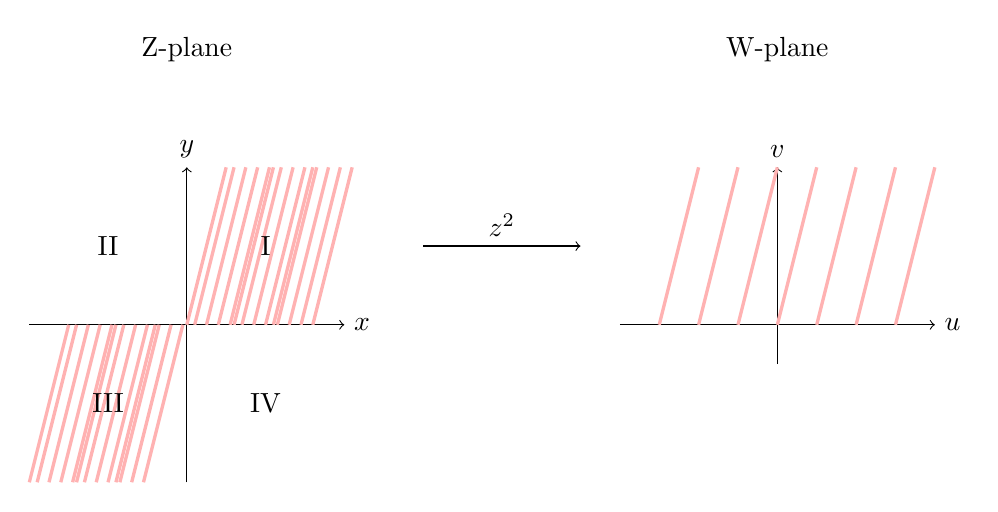
\begin{tikzpicture}

% Z-plane
\begin{scope}
    \node at (0,3.5) {Z-plane};
    \draw[->] (-2,0) -- (2,0) node[right] {$x$};
    \draw[->] (0,-2) -- (0,2) node[above] {$y$};

    % Shaded regions
   % \fill[red!30] (0,0) -- (2,0) -- (2,2) -- (0,2) -- cycle;
   % \fill[red!30] (-2,0) -- (0,0) -- (0,-2) -- (-2,-2) -- cycle;

	\foreach \x in {0,0.1, 0.25, 0.4, 0.55, 0.6, 0.7, 0.85, 1, 1.1, 1.15, 1.3, 1.45, 1.6}
		\draw[red!30, very thick] (\x, 0) -- (\x + 0.5, 2);
		
	\foreach \x in {0,0.1, 0.25, 0.4, 0.55, 0.6, 0.7, 0.85, 1, 1.1, 1.15, 1.3, 1.45}
		\draw[red!30, very thick] (\x-2,-2) -- (\x-2 + 0.5, 2-2);
    % Region labels
    \node at (1,1) {I};
    \node at (-1,1) {II};
    \node at (-1,-1) {III};
    \node at (1,-1) {IV};
\end{scope}

% Transformation arrow
\draw[->] (3,1) -- (5,1) node[midway, above] {$z^2$};

% W-plane
\begin{scope}[shift={(7.5,0)}]
    \node at (0,3.5) {W-plane};
    \draw[->] (-2,0) -- (2,0) node[right] {$u$};
    \draw[->] (0,-0.5) -- (0,2) node[above] {$v$};

    % Shaded region (approximate)
    \foreach \x in {-1.5,-1,...,1.5}
        \draw[red!30, very thick] (\x,2-2) -- (\x+0.5,2);

\end{scope}

\end{tikzpicture}

\end{document}